% Projekt: IFJ15 (Interpret jazyka) 
% Autor: Patrik Jurnečka
% Login: xjurne03
% Email: xjurne03@stud.fit.vutbr.cz
% Datum: 

\documentclass[a4paper, 11pt, titlepage]{article}
% Preambule
\usepackage[left=2cm, text={17cm, 24cm}, top=3cm]{geometry} %Rozmery
\usepackage{times} %Styl jazyka
\usepackage[IL2]{fontenc}
\usepackage[czech]{babel} %Jazyk
\usepackage[utf8]{inputenc} %Kodovani
\usepackage{graphics}
\usepackage{picture} 
\bibliographystyle{czplain}

\providecommand{\uv}[1]{\quotedblbase #1\textquotedblleft} %Uvozovky 

\begin{document} %Textova cast

\begin{titlepage} %Titulni strana
\begin{center}
\textsc{\Huge{Vysoké učení technické v~Brně}\\[3mm]\huge{Fakulta informačních technologií}}\\

\vspace{\stretch{0.1}}

\begin{figure}[h]
	\centering
	\scalebox{0.17}{\includegraphics{FIT_zakladni_provedeni_loga.jpg}}
\end{figure}

\vspace{\stretch{0.042}}
\huge{Dokumentace projektu do předmětu IFJ a IAL}\\
\Huge{\textbf{Interpret jazyka IFJ15}}\\
\LARGE{Tým 043, varianta b/2/I}
\vspace{\stretch{0.618}}
\end{center}

{\noindent\Large \hfill Martin Honza (xhonza03)\\}
{\indent\Large \hfill Patrik Jurnečka (xjurne03)\\}
{\indent\Large \hfill Hana Slámová (xslamo00)\\}
{\indent\Large \hfill Frantisek Šumšal (xsumsa01)\\}
{\indent\Large\today \hfill Adam Švidroň (xsvidr00)}

\end{titlepage}

\tableofcontents

\newpage

\section{Úvod} %Uvod
Dokumentace popisuje návrh a implementaci projektu Interpret jazyka IFJ15 do předmětu IFJ (Formální jazyky a~překladače) a IAL (Algoritmy). Vybrali jsme si zadání b/2/I, které nám udávalo, jáký algoritmus máme pro daný problém využít. Pro vyhledávání \textbf{Boyer-Mooreův algoritmus}, pro řazení algoritmus Heap sort, který byl využit ve vestavěné funkci \textbf{sort}. Poslední ze specifikových pravidel použití, jsme měli využít k implementaci tabulky symbolů \textbf{binární vyhledávací strom}. 

Cílem projektu bylo vytvořit program, který interpretuje jazyk IFJ15, což je velmi zjednodušenou podmnožinou jazyka C++11. 

\section{Struktura projektu}
Překladač je rozdělen do tří hlavních celků. Pomocí \textbf{lexikálního analyzátoru} načítá zdrojový kód. \textbf{Syntaktický analyzátor} zažádá lexikální o token a ověří syntaxi a sémantiku. Po bezchybné kontrole se spustí \textbf{interpret}.  

\section{Lexikální analizátor (scanner)}
Lexikální analyzátor načítá zdrojový kód po znacích a převádí jej na tokeny (funkce \textit{lex\_get\_token}), přičemž veškeré komentáře ignoruje. Implementováno pomocí konečného automatu (Obrázek~\ref{picture_1:konecny_automat}). Funkce je volána vždy, když syntaktický analizátor zažádá o~token. 

\subsection{Konečný automat}

\begin{figure}[h]
	\centering
	\scalebox{0.2}{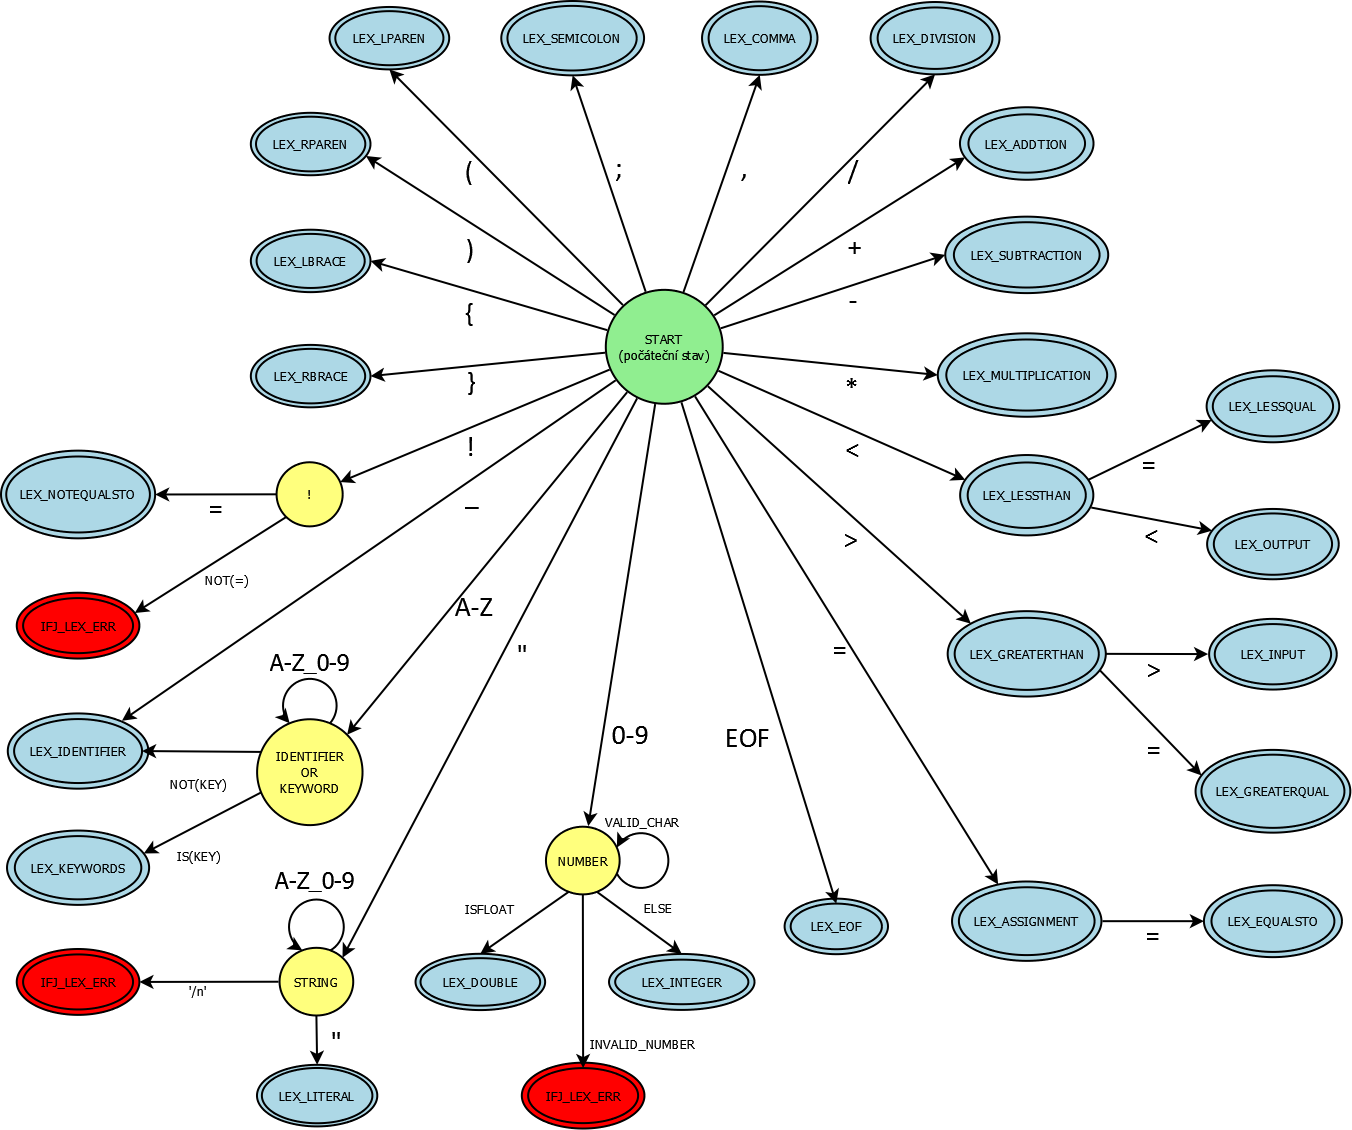
\includegraphics{konecny_automat.png}}
	\caption{Konečný automat}
	\label{picture_1:konecny_automat}
\end{figure}

\section{Syntaktická analizátor (parser)}
Syntaktický analyzátor postupně volá tokeny z lexikálního analyzátoru. Tokeny jsou zpracovávaný dvěma způsoby. Pomocí LL gramatiky (Tabulka \ref{table_1:LL_gramatic}) a precedenční syntaktické analýzy (Tabulka \ref{table_2:PA}). Při úspěšném dokončení syntaktické analýzy se generuje instrukční páska pro interpret.

\subsection{LL gramatika}
LL gramatika postupně ověřuje příchozí tokeny.   

\begin{table}[h]
\footnotesize
	\begin{center}
	\begin{tabular}{c c l}
	1.  & $<program>$ 	 & 	$<declrList>$ EOF \\ 
	2.  & $<declrList>$  &  $<funcDeclr>$ $<declrList>$ \\ 
	3.  & $<declrList>$  &  $<empty>$ \\ 
	4.  & $<funcDeclr>$  &  $<typeSpec>$ ID ($<params>$) \\
	5.  & $<typeSpec>$ 	 &  INT \\
	6.  & $<typeSpec>$   &  DOUBLE \\ 
	7.  & $<typeSpec>$ 	 &  STRING \\ 
	8.  & $<params>$ 	 & 	$<paramItem>$ \\ 
	9.  & $<params>$ 	 & 	$<paramItem>$, $<params>$ \\ 
	10. & $<paramItem>$  & 	$<typeSpec>$ ID\\ 
	11. & $<paramItem>$  & 	$<empty>$ \\ 
	\end{tabular}
	\caption{LL gramatika}
	\label{table_1:LL_gramatic}
	\end{center}
\end{table}

\subsection{Precedenční syntaktická analýza}
\begin{table}[h]
	\begin{center}
	\begin{tabular}{l | c c c c c c c c c c c c c c}
			  & $+$ & $-$ & $*$ & $/$ & $<$ & $>$ & $<=$& $>=$& $==$ & !$=$ &  $($   &  $)$   &  id  &    \$ \\ \hline
		$+$   & $>$ & $>$ & $<$ & $<$ & $>$ & $>$ & $>$ & $>$ & $>$  & $>$  & $<$  & $>$  & $<$  & $>$ \\
		$-$   & $>$ & $>$ & $<$ & $<$ & $>$ & $>$ & $>$ & $>$ & $>$  & $>$  & $<$  & $>$  & $<$  & $>$ \\
		$*$   & $>$ & $>$ & $>$ & $>$ & $>$ & $>$ & $>$ & $>$ & $>$  & $>$  & $<$  & $>$  & $<$  & $>$ \\
		$/$   & $>$ & $>$ & $>$ & $>$ & $>$ & $>$ & $>$ & $>$ & $>$  & $>$  & $<$  & $>$  & $<$  & $>$ \\
		$<$   & $<$ & $<$ & $<$ & $<$ & $<$ & $>$ & $>$ & $>$ & $>$  & $>$  & $<$  & $>$  & $<$  & $>$ \\
		$>$   & $<$ & $<$ & $<$ & $<$ & $<$ & $>$ & $>$ & $>$ & $>$  & $>$  & $<$  & $>$  & $<$  & $>$ \\
		$<=$  & $<$ & $<$ & $<$ & $<$ & $<$ & $>$ & $>$ & $>$ & $>$  & $>$  & $<$  & $>$  & $<$  & $>$ \\
		$>=$  & $<$ & $<$ & $<$ & $<$ & $<$ & $>$ & $>$ & $>$ & $>$  & $>$  & $<$  & $>$  & $<$  & $>$ \\
		$==$  & $<$ & $<$ & $<$ & $<$ & $<$ & $>$ & $>$ & $>$ & $>$  & $>$  & $<$  & $>$  & $<$  & $>$ \\
		!$=$  & $<$ & $<$ & $<$ & $<$ & $>$ & $>$ & $>$ & $>$ & $>$  & $>$  & $<$  & $>$  & $<$  & $>$ \\
		$($   & $<$ & $<$ & $<$ & $<$ & $<$ & $<$ & $<$ & $<$ & $<$  & $<$  & $<$  & $=$  & $<$  &     \\
		$)$   & $>$ & $>$ & $>$ & $>$ & $>$ & $>$ & $>$ & $>$ & $>$  & $>$  &      & $>$  &      & $>$ \\
		id    & $>$ & $>$ & $>$ & $>$ & $>$ & $>$ & $>$ & $>$ & $>$  & $>$  &      & $>$  &      & $>$ \\
		\$    & $<$ & $<$ & $<$ & $<$ & $<$ & $<$ & $<$ & $<$ & $<$  & $<$  & $<$  &      & $<$  &     \\ \hline
	\end{tabular}
	\caption{Precenenční tabulka syntaktické analýzy výrazů}
	\label{table_2:PA}
	\end{center}
\end{table}

\section{Sémantický analizátor}

\section{Interpret}

\newpage

\section{Algoritmy z předmětu IAL}

\subsection{Heapsort}
\subsection{Boyer-Mooreův algoritmus}
\subsection{Binární vyhledávací strom (BVS)}

\newpage

\section{Práce v týmu}
\subsection{Rozdělení práce}

\begin{itemize}
	\item\textbf{Martin Honza:}
	\item\textbf{Patrik Jurnečka:} Syntaktický analyzátor, dokumentace
	\item\textbf{Hana Slámová:} Vestavěné funkce
	\item\textbf{Frantisek Šumšal:} Lexikální analýzátor, syntaktický analyzátor
	\item\textbf{Adam Švidroň:} Heap sort
\end{itemize}  

\section{Závěr}
\subsection{Metriky kódu}

\section{Literatura}

\bibliography{literatura}

\end{document} %konec textove casti